%%%%%%%%%%%%%%%%%%%%%%%%%%%%%%%%%%%%%%%%%
% Short Sectioned Assignment LaTeX Template Version 1.0 (5/5/12)
% This template has been downloaded from: http://www.LaTeXTemplates.com
% Original author:  Frits Wenneker (http://www.howtotex.com)
% License: CC BY-NC-SA 3.0 (http://creativecommons.org/licenses/by-nc-sa/3.0/)
%%%%%%%%%%%%%%%%%%%%%%%%%%%%%%%%%%%%%%%%%

%----------------------------------------------------------------------------------------
%	PACKAGES AND OTHER DOCUMENT CONFIGURATIONS
%----------------------------------------------------------------------------------------

\documentclass[paper=a4, fontsize=11pt]{scrartcl} % A4 paper and 11pt font size

% ---- Entrada y salida de texto -----

\usepackage[T1]{fontenc} % Use 8-bit encoding that has 256 glyphs
\usepackage[utf8]{inputenc}
%\usepackage{fourier} % Use the Adobe Utopia font for the document - comment this line to return to the LaTeX default

% ---- Idioma --------

\usepackage[spanish, es-tabla]{babel} % Selecciona el español para palabras introducidas automáticamente, p.ej. "septiembre" en la fecha y especifica que se use la palabra Tabla en vez de Cuadro

\usepackage{eurosym}
\usepackage{enumitem}

% ---- Otros paquetes ----

\usepackage{url} % ,href} %para incluir URLs e hipervínculos dentro del texto (aunque hay que instalar href)
\usepackage{amsmath,amsfonts,amsthm} % Math packages
%\usepackage{graphics,graphicx, floatrow} %para incluir imágenes y notas en las imágenes
\usepackage{graphics,graphicx, float} %para incluir imágenes y colocarlas

% Para hacer tablas comlejas
%\usepackage{multirow}
%\usepackage{threeparttable}

%\usepackage{sectsty} % Allows customizing section commands
%\allsectionsfont{\centering \normalfont\scshape} % Make all sections centered, the default font and small caps

\usepackage{fancyhdr} % Custom headers and footers
\pagestyle{fancyplain} % Makes all pages in the document conform to the custom headers and footers
\fancyhead{} % No page header - if you want one, create it in the same way as the footers below
\fancyfoot[L]{} % Empty left footer
\fancyfoot[C]{} % Empty center footer
\fancyfoot[R]{\thepage} % Page numbering for right footer
\renewcommand{\headrulewidth}{0pt} % Remove header underlines
\renewcommand{\footrulewidth}{0pt} % Remove footer underlines
\setlength{\headheight}{13.6pt} % Customize the height of the header

\numberwithin{equation}{section} % Number equations within sections (i.e. 1.1, 1.2, 2.1, 2.2 instead of 1, 2, 3, 4)
\numberwithin{figure}{section} % Number figures within sections (i.e. 1.1, 1.2, 2.1, 2.2 instead of 1, 2, 3, 4)
\numberwithin{table}{section} % Number tables within sections (i.e. 1.1, 1.2, 2.1, 2.2 instead of 1, 2, 3, 4)

\setlength\parindent{0pt} % Removes all indentation from paragraphs - comment this line for an assignment with lots of text

\newcommand{\horrule}[1]{\rule{\linewidth}{#1}} % Create horizontal rule command with 1 argument of height


%----------------------------------------------------------------------------------------
%	TÍTULO Y DATOS DEL ALUMNO
%----------------------------------------------------------------------------------------

\title{	
\normalfont \normalsize 
\textsc{\textbf{Ingeniería de Servidores (2016-2017)} \\ Grado en Ingeniería Informática \\ Universidad de Granada} \\ [25pt] % Your university, school and/or department name(s)
\horrule{0.5pt} \\[0.4cm] % Thin top horizontal rule
\huge Memoria Práctica 1 \\ % The assignment title
\horrule{2pt} \\[0.5cm] % Thick bottom horizontal rule
}

\author{Cristian Vélez Ruiz} % Nombre y apellidos

\date{\normalsize\today} % Incluye la fecha actual

%----------------------------------------------------------------------------------------
% DOCUMENTO
%----------------------------------------------------------------------------------------

\begin{document}

\maketitle % Muestra el Título

\newpage %inserta un salto de página

\tableofcontents % para generar el índice de contenidos

\listoffigures

\listoftables

\newpage

%----------------------------------------------------------------------------------------
%	Cuestión 1
%----------------------------------------------------------------------------------------

\section{¿Qué modos y/o tipos de “virtualización” existen?}

\begin{itemize}
\item \textbf{Virtualización a nivel de aplicaciones:} Separa las aplicaciones del hardware y el software ,lo que nos ofrece migrar la aplicacion de una maquina a otra sin interrumpir otros sistemas.
\item \textbf{Virtualización a nivel de sistema operativo :}El servidor físico y una única instancia del SO son virtualizadas en varias particiones aisladas.
\item \textbf{Virtualización a nivel de hardware:} Consiste en emular distintos hardware dentro de un mismo hardware para poder repartir los recursos fisicos y se puedan usar mejor , una de las ventajas es que si una maquina necesita mas recursos se le puede dar de otra que no lo este utilizando.
\end{itemize}



%----------------------------------------------------------------------------------------
%	Cuestión 2
%----------------------------------------------------------------------------------------

\section{Muestre los precios y características de varios proveedores de VPS (Virtual Private Server) y compare con el precio de servidores dedicados (administrados y no administrados). Comente diferencias.}

\begin{table}[H]
	\centering
	\begin{tabular}{|c|c|c|}
		\hline
		\textbf{	} & \textbf{Administrado} & \textbf{No Administrado} \\
		\hline
		Dedicado & 198\textup{\euro} & 99\textup{\euro} \\
		\hline
		Virtual & 126\textup{\euro} & 27\textup{\euro} \\
		\hline
	\end{tabular}  
	\caption{Precios por de servidores parecidos en Hostalia} \label{tab:tablaPrecios}
\end{table}

En casi toda la administración de servidores, ya sea dedicado o virtual, hostalia \cite{hostalia} cobra una tarifa de 99\textup{\euro} al mes , como también se puede observar lo que mas económico nos saldría seria un servidor virtual gestionado por nosotros mismos.

Las limitaciones que nos ponen en los servidores virtuales son tasas máximas de transferencia , es una de las desventajas , aunque si aumentas el plan estas también aumentan.


%----------------------------------------------------------------------------------------
%	Cuestión 3
%----------------------------------------------------------------------------------------

\section{a) Enumere y explique brevemente al menos tres de las innovaciones en Windows Server 2016 y 2012 R2 respecto a 2008R2. b)¿Qué es Windows Server 2016 nano?}

\begin{enumerate}[label=(\alph*)]
	\item Windows 2012 R2 puede tener hasta una almacenamiento físico de hasta 4Tb mientras que 2008 R2 solo tiene hasta 1Tb \cite{comparacionMicroSer}.
	
	Windows 2012 R2 tiene soporte de hasta 320 procesadores lógicos y Windows 2008 R2 hasta 64 \cite{comparacionMicroSer}.
	
	Windows 2012 R2 soporta hasta 64 procesadores virtuales por maquina virtual , mientras que Windows 2008 R2 solamente 4 \cite{comparacionMicroSer}.
	
	\item  Windows Server 2016 nano es una nueva versión de Windows Server en la cual han reducido su instalación base hasta ocupar unos 200 Mb aproximadamente , eliminando la interfaz gráfica , lo cual el servidor se tendrá que administras mediante PowerShell o Remote Server Managment. También han reducido la probabilidad de tener que realizar un reinicio después de instalar ciertas instalaciones \cite{nanoServer}.
	
	
\end{enumerate}


%----------------------------------------------------------------------------------------
%	Cuestión 4
%----------------------------------------------------------------------------------------

\section{¿Qué son los productos MAAS y Landscape ofrecidos por Canonical (la empresa que desarrolla Ubuntu)?}

%------------------------------------------------
\begin{itemize}
	\item \textbf{MAAS:} Nos ofrece un control sobre cada maquina física , donde podemos cambiar su Sistema Operativo, a nuestra conveniencia con una imagen personalizada en cuestión de unos pocos clics y en cuestión de minutos ya estará instalada, una buena herramienta para escalar dependiendo de las necesidades en tiempo real , ya que podemos ver los recursos de cada una . 
	
	Herramienta gratuita para Ubuntu y CentOS pero sin soporte , si queremos otros SO , o soporte tienen distintos planes \cite{maas}.
	
	\item \textbf{Landscape:} Permite poder actualizar múltiples maquinas desde el mismo programa,ya sean Pcs de escritorio , servidores o maquinas virtuales , automatizar actualizaciones, y crear repositorios propios para nuestro software, es una herramienta de pago \cite{landscape}.
\end{itemize}

\section{¿Qué relación tiene esta distribución con Red Hat y con el proyecto Fedora?}
Red Hat fue creado para profesionales y empresas con soporte , pero Fedora se crea a partir de Red Hat y es desarrollada y mantenida por la comunidad, ambas son de código abierto.
\section{¿Qué diferencias hay entre RAID mediante SW y mediante HW?}

En un Raid mediante software la redundancia y la escritura/lectura la tiene que tener controlada el Sistema Operativo , pero en Hardware se comporta como un solo disco y el hardware se encarga de hacer toda la gestión

\section{a) ¿Qué es LVM? b)¿Qué ventaja tiene para un servidor de gama baja? c) Si va a tener un servidor web, ¿le daría un tamaño grande o pequeño a /var?}

\begin{enumerate}[label=(\alph*)]
	\item LVM es un gestor de Volúmenes Lógicos para los kernels de Linux
	\item Para un servidor de gama baja una ventaja seria que si nos quedamos sin memoria , podríamos ampliarla sin necesidad de volver a particionar físicamente , ya que si están dentro del mismo MD se pueden modificar sus tamaños , e incluso dar a unas particiones el espacio que otras no utilizan.
	
	 En un servidor le daría un espacio mas grande , ya que contiene datos que cambian cuando el sistema se ejecuta , por eso al hacer solicitudes de ciertas cosas a un servidor tendrán que ir cambiando y necesitar un mayor espacio.
\end{enumerate}

\section{¿Debemos cifrar también el volumen que contiene el espacio	para swap? ¿y el volumen en el que montaremos /boot?}

El volumen swap debe estar cifrado para evitar volcados de memoria y puedan extraer información . 

/boot no puede estar cifrada porque entonces no podremos arrancar el SO ya que los datos de arranque estarán cifrados.

\section{a)Imagine que tiene un disco híbrido con tecnología SSD ¿Qué puntos de montaje ubicaría en este? b) Justifique qué tipo de sistema de archivos usaría para tener un servidor de streaming}

\begin{enumerate}[label=(\alph*)]
	\item En la ubicación del SSD estableceremos la partición / , para que todos los programas puedan cargar rápido, /boot para un arranque rápido, /var para poder almacenar los datos de los programas ,/tmp para el uso de archivos temporales y en la parte del HDD estableceremos la partición /home para ubicar los datos personales y otros mas pesados.
	\item Un servidor de streaming necesita manejar grandes archivos como por ejemplo puede ser un vídeo en 4K , o en 360 grados , por lo que necesitara un sistema de archivos que pueda manejar grandes datos como por ejemplo Ext4, NTFS o XFS.
\end{enumerate}

\section{Muestre cómo ha quedado el disco particionado una vez el sistema está instalado y ha iniciado sesión. (comando: lsblk)}

	\begin{figure}[H] %con el [H] le obligamos a situar aquí la figura
		\centering
		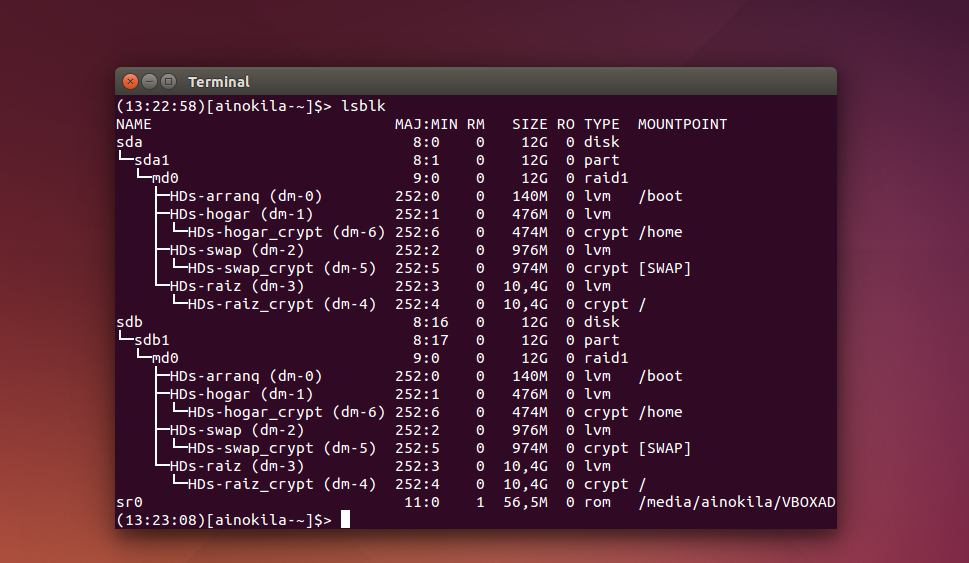
\includegraphics[scale=0.5]{pics/Captura10.png}  %el parámetro scale permite agrandar o achicar la imagen. En el nombre de archivo puede especificar directorios
		\caption{Estado de los discos del sistema} \label{fig:figura10}
	\end{figure}

	Como se puede apreciar las particiones sda1 y sdb1 tienen una estructura de particiones idénticas , debido a la configuración en Raid 1 que hemos hecho.



\section{a) ¿Cómo ha hecho el disco 2 “arrancable”? b) ¿Qué hace el comando grub-install?}

\begin{enumerate}[label=(\alph*)]
	\item sudo grub-install sdb ,después tenemos que arreglar el bug que tiene Ubuntu , ya que si falla el disco 2 seguiría funcionando , pero si se rompe el 1 disco no funcionara , para conseguirlo :
	\begin{itemize}
		\item cat /proc/mdstat Nos muestra que el disco esta inactivo , aunque debería aparecer como degradado debido al bug.
		\item Utilizaremos mdadm (gestión de multi-dispositivos) lo forzaremos que lo active.
		\item mdadm -R /dev/md0
		\item cat /proc/mdstat ahora nos muestra que esta activo.
	\end{itemize}
	\item Es un comando para instalar el Gestor de Arranque de Linux. \cite{grub}
\end{enumerate}


\section[Opcional 1]{Muestre (con capturas de pantalla) cómo ha comprobado que el RAID1 funciona.}

	\begin{figure}[H] %con el [H] le obligamos a situar aquí la figura
			\centering
			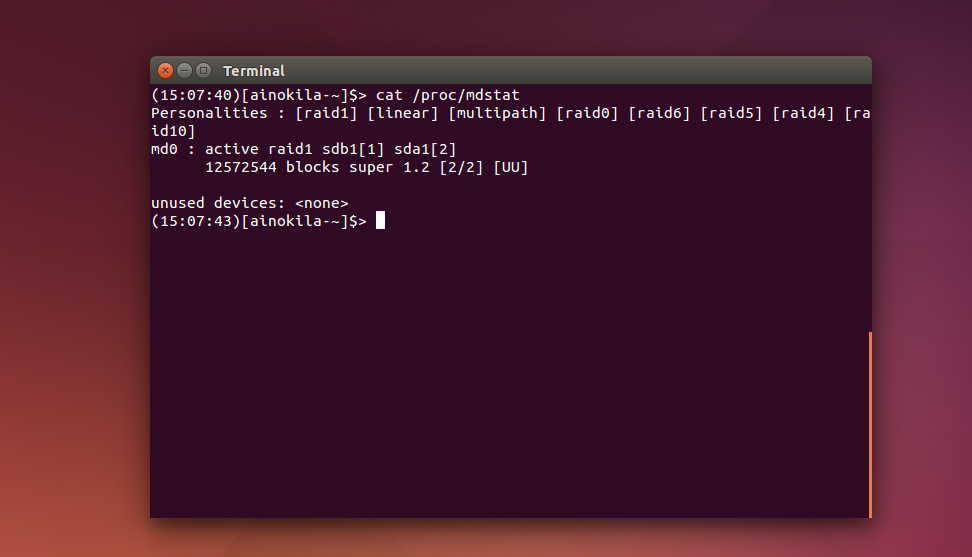
\includegraphics[scale=0.5]{pics/Captura11.png}  %el parámetro scale permite agrandar o achicar la imagen. En el nombre de archivo puede especificar directorios
			\caption{Estado del de Raid} \label{fig:figura11}
	\end{figure}

	Como se puede observar nos dice que esta activo y que raid1 esta formado por  sdb1 y sda1, y ambos están en funcionamiento debido a las dos U , en caso contrario aparecería un guion bajo.
	
	

\section{¿Qué diferencia hay entre Standard y Datacenter?}

Ambas ediciones de Windows Server nos proporcionan las mismas características, la única diferencia entre ellas es el numero de maquinas virtuales que son capaces de ejecutar, ya que en la edición Standar el numero de MVs es de 2, a ejecutar en hasta 2 procesadores , mientras que la versión Datacenter su numero es ilimitado \cite{datacenterystandar}.

\section{Continúe usted con el proceso de definición de RAID1 para los dos discos de 50MiB que ha creado. Muestre el proceso con capturas de pantalla.}

	\begin{itemize}
		\item Vamos encima de PC y damos botón derecho , seguidamente a Administrar
		\begin{figure}[H] %con el [H] le obligamos a situar aquí la figura
			\centering
			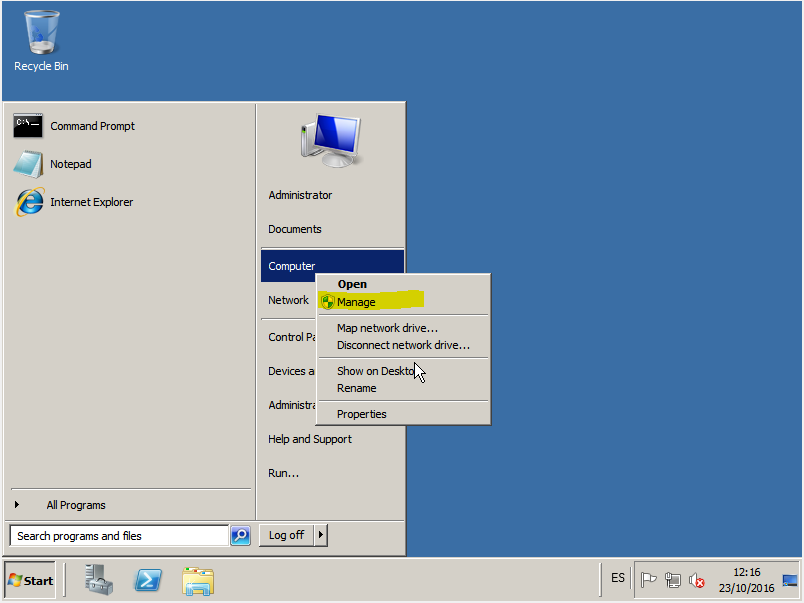
\includegraphics[scale=0.5]{pics/Captura1.png}  %el parámetro scale permite agrandar o achicar la imagen. En el nombre de archivo puede especificar directorios
			\caption{Creación de Raid 1 : Paso 1} \label{fig:figura1}
		\end{figure}
		
		\item Nos mostrara los discos que detecta el SO , seleccionaremos uno de los dos discos de 25Mib.
		\begin{figure}[H] %con el [H] le obligamos a situar aquí la figura
			\centering
			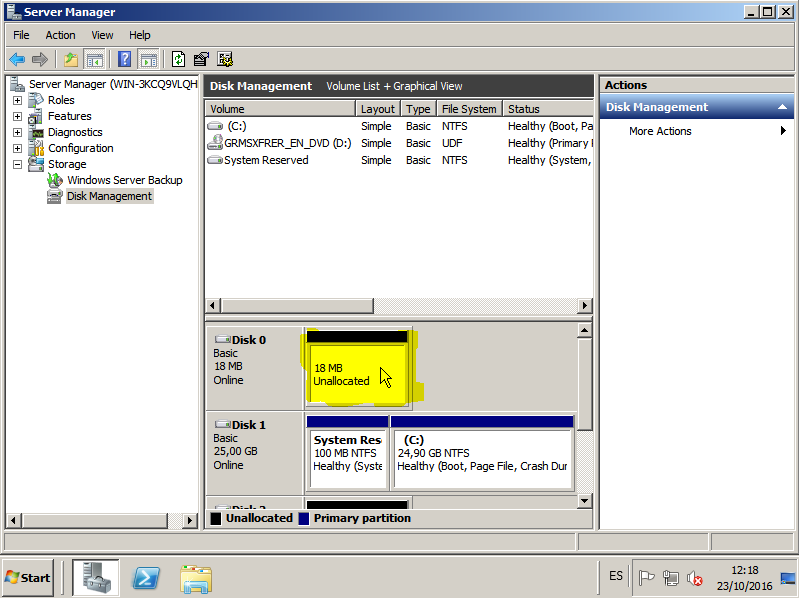
\includegraphics[scale=0.5]{pics/Captura2.png}  %el parámetro scale permite agrandar o achicar la imagen. En el nombre de archivo puede especificar directorios
			\caption{Creación de Raid 1 : Paso 2} \label{fig:figura2}
		\end{figure}
	
		\item Ahora seleccionamos crear un volumen en modo espejo. Sistema Raid en Windows 
		\begin{figure}[H] %con el [H] le obligamos a situar aquí la figura
			\centering
			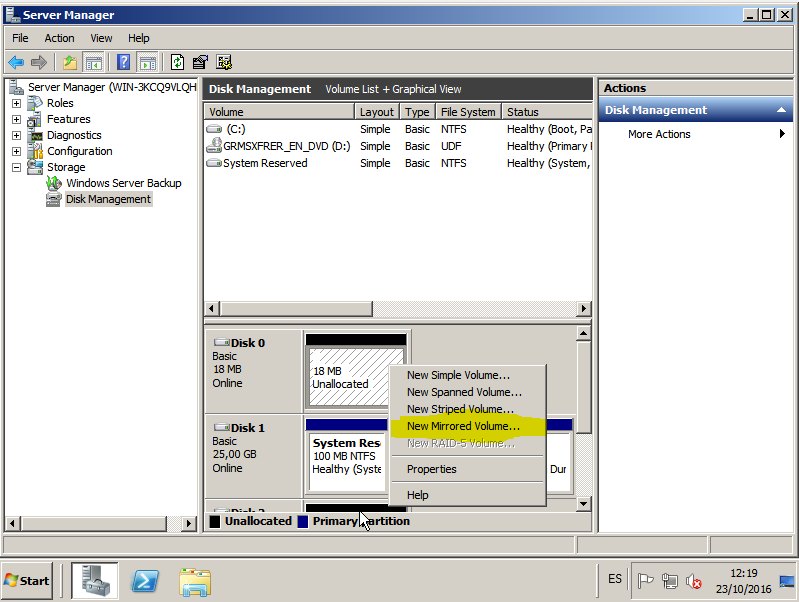
\includegraphics[scale=0.5]{pics/Captura3.png}  %el parámetro scale permite agrandar o achicar la imagen. En el nombre de archivo puede especificar directorios
			\caption{Creación de Raid 1 : Paso 3} \label{fig:figura3}
		\end{figure}
	
		\item Seleccionamos el disco que antes quedo sin seleccionar y le damos a añadir.
		\begin{figure}[H] %con el [H] le obligamos a situar aquí la figura
			\centering
			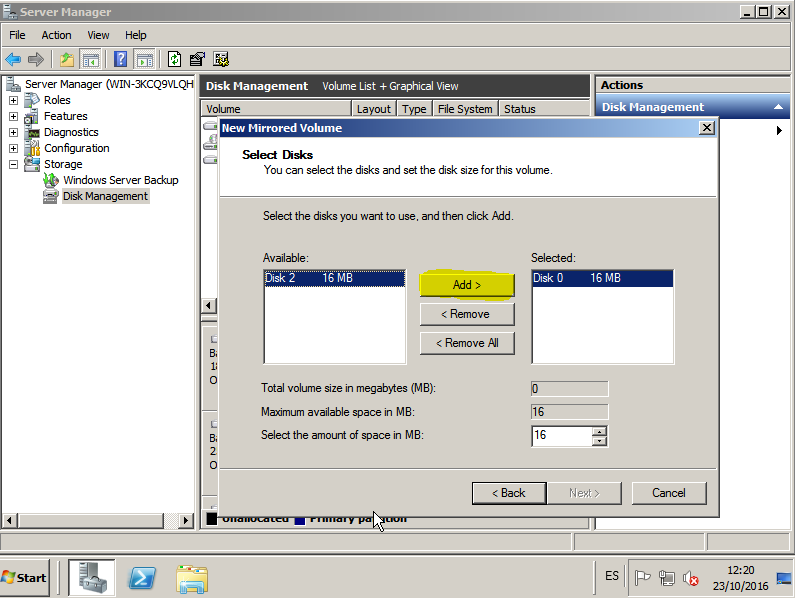
\includegraphics[scale=0.5]{pics/Captura4.png}  %el parámetro scale permite agrandar o achicar la imagen. En el nombre de archivo puede especificar directorios
			\caption{Creación de Raid 1 : Paso 4} \label{fig:figura4}
		\end{figure}
	
		\item Debe quedar de esta manera , los dos discos que formaran el Raid en el lado derecho.
		\begin{figure}[H] %con el [H] le obligamos a situar aquí la figura
			\centering
			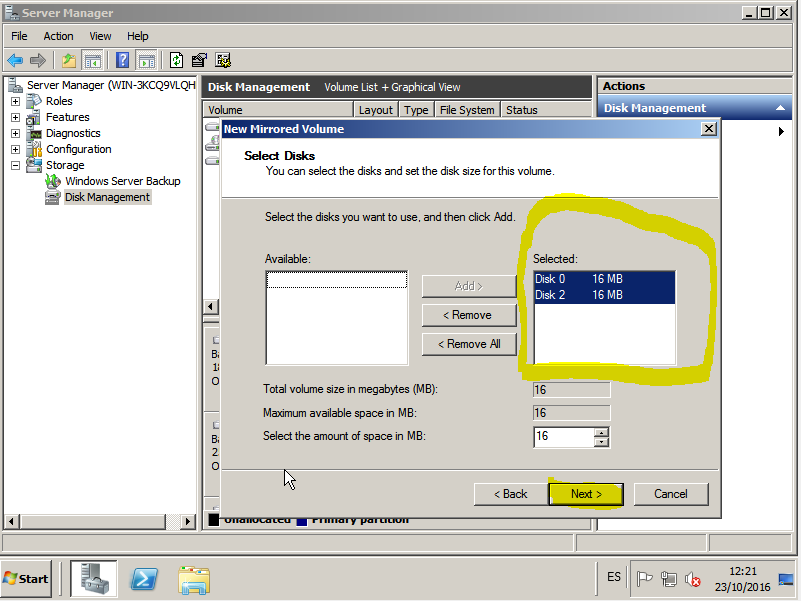
\includegraphics[scale=0.5]{pics/Captura5.png}  %el parámetro scale permite agrandar o achicar la imagen. En el nombre de archivo puede especificar directorios
			\caption{Creación de Raid 1 : Paso 5} \label{fig:figura5}
		\end{figure}
	
		\item Asignamos la letra al nuevo volumen y le damos a siguiente.
		\begin{figure}[H] %con el [H] le obligamos a situar aquí la figura
			\centering
			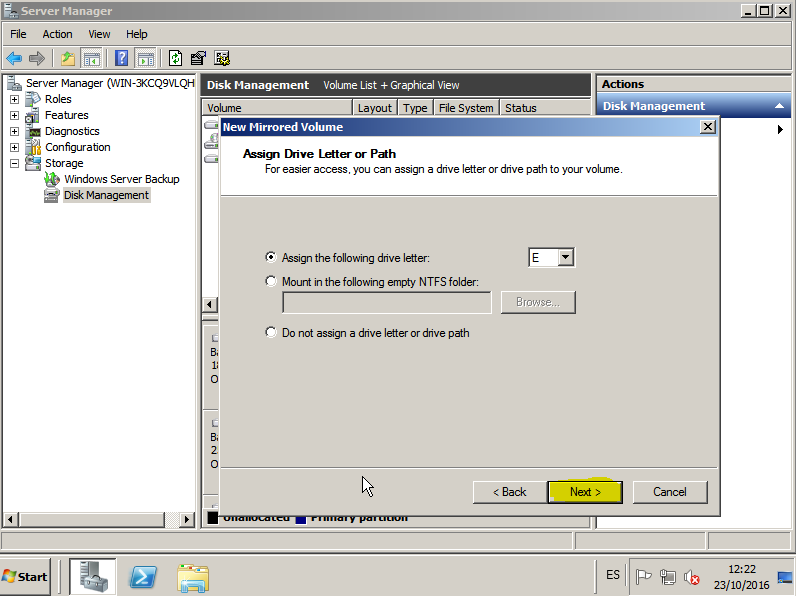
\includegraphics[scale=0.5]{pics/Captura6.png}  %el parámetro scale permite agrandar o achicar la imagen. En el nombre de archivo puede especificar directorios
			\caption{Creación de Raid 1 : Paso 6} \label{fig:figura6}
		\end{figure}
	
		\item Asignamos el sistema de archivos que queramos que use , y el nombre del volumen , en nuestro caso Raid 1.	
		\begin{figure}[H] %con el [H] le obligamos a situar aquí la figura
			\centering
			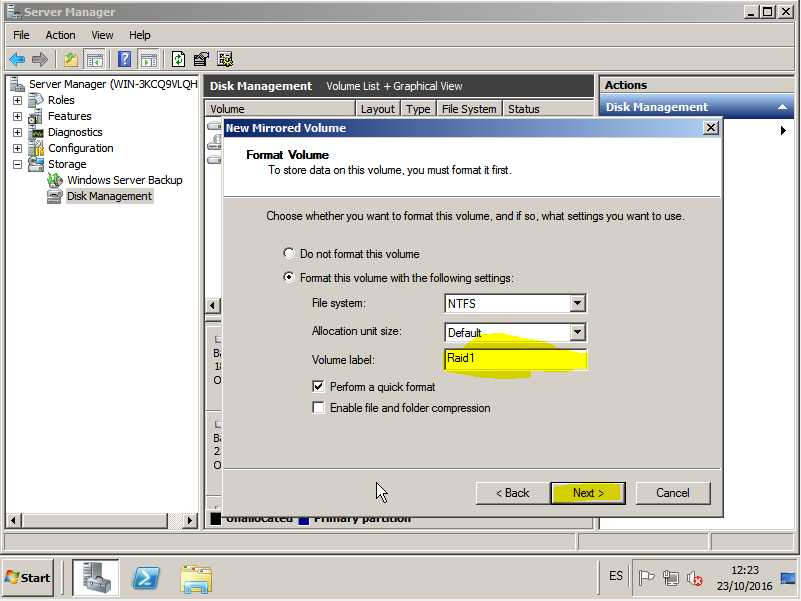
\includegraphics[scale=0.5]{pics/Captura7.png}  %el parámetro scale permite agrandar o achicar la imagen. En el nombre de archivo puede especificar directorios
			\caption{Creación de Raid 1 : Paso 7} \label{fig:figura7}
		\end{figure}
	
		\item Nos muestra el resumen de la accion a aplicar , si todo es correcto le damos a finalizar.	
		\begin{figure}[H] %con el [H] le obligamos a situar aquí la figura
			\centering
			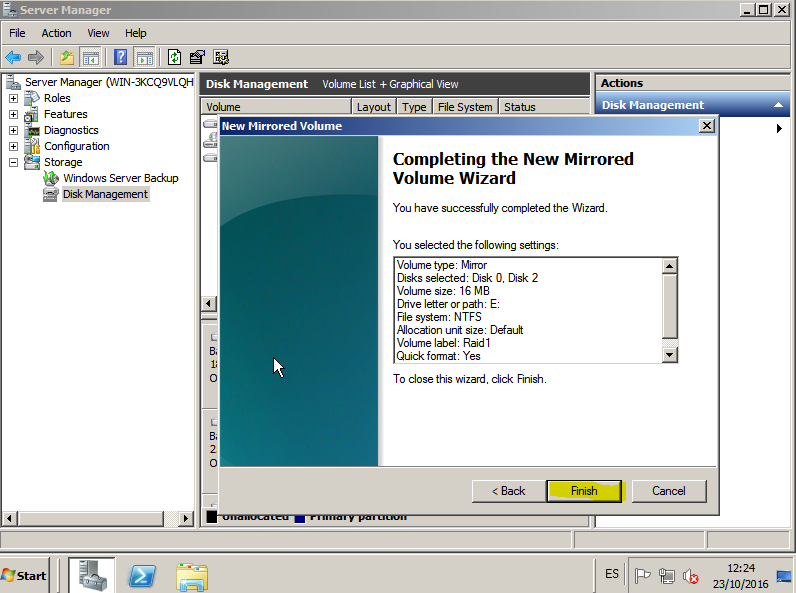
\includegraphics[scale=0.5]{pics/Captura8.png}  %el parámetro scale permite agrandar o achicar la imagen. En el nombre de archivo puede especificar directorios
			\caption{Creación de Raid 1 : Paso 8} \label{fig:figura8}
		\end{figure}
	
		\item Ahora nuestros discos han quedado de la siguiente manera.
		\begin{figure}[H] %con el [H] le obligamos a situar aquí la figura
			\centering
			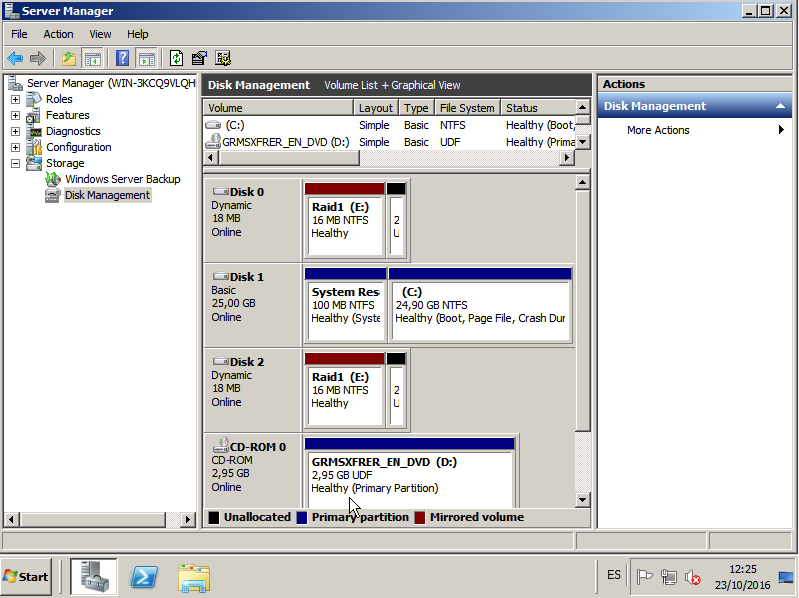
\includegraphics[scale=0.5]{pics/Captura9.png}  %el parámetro scale permite agrandar o achicar la imagen. En el nombre de archivo puede especificar directorios
			\caption{Creación de Raid 1 : Paso 9} \label{fig:figura9}
		\end{figure}
	
	\end{itemize}
	


\section{Explique brevemente qué diferencias hay entre los tres tipos de conexión que permite el VMSW para las Mvs: NAT, Host-only y Bridge.}

\begin{itemize}
	\item \textbf{NAT}: Enmascara toda la información que proviene de la maquina virtual como si fuese del host anfitrión , tiene conexión al exterior gracias a eso \cite{red}.
	\item \textbf{Host-Only}: Nos permite solo la comunicación con el Host anfitrión y con las demás maquinas virtuales, no permite conexión fuera de esa red o a Internet \cite{red}.
	\item \textbf{Bridge}: Usa la tarjeta de red del ordenador anfitrión y es otro dispositivo mas conectado a la red real \cite{red}.
\end{itemize}

\section[Opcional 2]{¿Qué relación hay entre los atajos de teclado de emacs y los de la consola bash? ¿y entre los de vi y las páginas del manual?}

\begin{itemize}
	\item Son muy similares , internamente emacs tiene un interprete de comandos que son los que utiliza bash. 
	
\end{itemize}


%------------------------------------------------

\bibliography{citas} %archivo citas.bib que contiene las entradas 
\bibliographystyle{plain} % hay varias formas de citar

\end{document}
